\documentclass[10pt,journal]{IEEEtran}
\usepackage[T1]{fontenc}
\usepackage{newtxtext,newtxmath}
\usepackage{amsmath,booktabs,graphicx,siunitx,hyperref,fancyhdr,xcolor,cite}
\sisetup{detect-all}
\hypersetup{hidelinks}
\graphicspath{{figures/}}
\fancypagestyle{paper}{\fancyhf{}\fancyfoot[R]{\thepage}\renewcommand{\headrulewidth}{0pt}}
\fancypagestyle{IEEEtitlepagestyle}{\fancyhf{}\fancyfoot[R]{\thepage}\renewcommand{\headrulewidth}{0pt}}
\pagestyle{paper}
% Float placement: never leave a sliver of text under a stack of figures; prefer a clean float page.
\renewcommand{\topfraction}{0.85}\renewcommand{\dbltopfraction}{0.85}
\renewcommand{\textfraction}{0.2}\renewcommand{\floatpagefraction}{0.7}\renewcommand{\dblfloatpagefraction}{0.7}
\setcounter{topnumber}{2}\setcounter{dbltopnumber}{2}
% Auto-generated by export_plot_data.py -- do not edit.
\newcommand{\nJepaH}{10.1}
\newcommand{\nJepaHsd}{\textbf{n/a}}
\newcommand{\nJepaMlpH}{9.0}
\newcommand{\nReconH}{17.3}
\newcommand{\nReconMlpH}{11.6}
\newcommand{\nSupAllH}{7.3}
\newcommand{\nSupThreeH}{14.7}
\newcommand{\nFtThreeH}{9.5}
\newcommand{\nGreyH}{4.6}
\newcommand{\nNominalH}{43.1}
\newcommand{\nGreyOOD}{7.6}
\newcommand{\nJepaOOD}{14.4}
\newcommand{\nSupAllOOD}{11.7}
\newcommand{\nGreyLamZero}{4.1}
\newcommand{\nGreyLamThree}{14.3}
\newcommand{\nJepaLamZero}{10.1}
\newcommand{\nJepaLamThree}{12.9}
\newcommand{\nReconLamThree}{21.2}
\newcommand{\nSupAllLamThree}{11.1}
\newcommand{\nSupThreeLamThree}{27.5}
\newcommand{\nFtThreeLamThree}{12.9}
\newcommand{\nJepaProbeTen}{11.9}
\newcommand{\nSupTen}{40.6}
\newcommand{\nFtTen}{18.9}
\newcommand{\nJepaFilt}{6.7}
\newcommand{\nJepaMlpFilt}{3.7}
\newcommand{\nReconFilt}{9.8}
\newcommand{\nSupAllFilt}{2.3}
\newcommand{\nTrackerFilt}{4.4}
\newcommand{\nGainJepa}{0.09}
\newcommand{\nGainRecon}{0.19}
\newcommand{\nGainSup}{0.04}
\newcommand{\nGainGrey}{0.03}
\newcommand{\nAblShort}{14.7}
\newcommand{\nAblRand}{15.7}
\newcommand{\nAblCtx}{16.1}
\newcommand{\nAblXlong}{\textbf{n/a}}
\newcommand{\nAblMix}{\textbf{n/a}}
\newcommand{\nAblMixLamThree}{\textbf{n/a}}
\newcommand{\nAblMixLamZero}{\textbf{n/a}}
\newcommand{\nAblHiLamThree}{\textbf{n/a}}
\newcommand{\nAblJepaSzLamThree}{12.9}
\newcommand{\nAblReconMixLamThree}{\textbf{n/a}}
\newcommand{\nLabelRatioTen}{3.4}
\newcommand{\nSeeds}{1}
\newcommand{\nRtwoKwJepa}{0.76}
\newcommand{\nRtwoTauJepa}{0.38}
\newcommand{\nRtwoTauSup}{0.61}
\newcommand{\nRtwoJJepa}{0.05}
\newcommand{\nMpcFtId}{7.7}
\newcommand{\nMpcSupThreeId}{22.2}
\newcommand{\nMpcGreyId}{6.6}
\newcommand{\nMpcJepaId}{7.9}
\newcommand{\nMpcReconId}{22.7}
\newcommand{\nMpcSupAllId}{3.9}
\newcommand{\nMpcPiId}{344}
\newcommand{\nMpcJepaHiId}{\textbf{n/a}}
\newcommand{\nMpcRatioId}{2.9}
\newcommand{\nMpcFtLamThree}{28.6}
\newcommand{\nMpcSupThreeLamThree}{224}
\newcommand{\nMpcGreyLamThree}{14.5}
\newcommand{\nMpcJepaLamThree}{38.6}
\newcommand{\nMpcReconLamThree}{85.8}
\newcommand{\nMpcSupAllLamThree}{20.8}
\newcommand{\nMpcPiLamThree}{2444}
\newcommand{\nMpcJepaHiLamThree}{\textbf{n/a}}
\newcommand{\nMpcRatioLamThree}{7.8}
\newcommand{\nHybJepaId}{7.0}
\newcommand{\nHybJepaOOD}{\textbf{n/a}}
\newcommand{\nHybJepaLamThree}{\textbf{n/a}}
\newcommand{\nHybJepaLamTwo}{\textbf{n/a}}
\newcommand{\nHybJepaLamZero}{\textbf{n/a}}
\newcommand{\nHybFtId}{\textbf{n/a}}
\newcommand{\nHybFtOOD}{\textbf{n/a}}
\newcommand{\nHybFtLamThree}{\textbf{n/a}}
\newcommand{\nHybFtLamTwo}{\textbf{n/a}}
\newcommand{\nHybFtLamZero}{\textbf{n/a}}
\newcommand{\nHybTrackerId}{5.9}
\newcommand{\nHybTrackerOOD}{\textbf{n/a}}
\newcommand{\nHybTrackerLamThree}{\textbf{n/a}}
\newcommand{\nHybTrackerLamTwo}{\textbf{n/a}}
\newcommand{\nHybTrackerLamZero}{\textbf{n/a}}
\newcommand{\nHybSupThreeId}{\textbf{n/a}}
\newcommand{\nHybSupThreeOOD}{\textbf{n/a}}
\newcommand{\nHybSupThreeLamThree}{\textbf{n/a}}
\newcommand{\nHybSupThreeLamTwo}{\textbf{n/a}}
\newcommand{\nHybSupThreeLamZero}{\textbf{n/a}}
\newcommand{\nEnsJepaId}{\textbf{n/a}}
\newcommand{\nEnsSingleJepaId}{\textbf{n/a}}
\newcommand{\nEnsCovJepaId}{\textbf{n/a}}
\newcommand{\nEnsCorrJepaId}{\textbf{n/a}}
\newcommand{\nEnsJepaLamThree}{\textbf{n/a}}
\newcommand{\nEnsSingleJepaLamThree}{\textbf{n/a}}
\newcommand{\nEnsCovJepaLamThree}{\textbf{n/a}}
\newcommand{\nEnsCorrJepaLamThree}{\textbf{n/a}}
\newcommand{\nEnsJepaOOD}{\textbf{n/a}}
\newcommand{\nEnsSingleJepaOOD}{\textbf{n/a}}
\newcommand{\nEnsCovJepaOOD}{\textbf{n/a}}
\newcommand{\nEnsCorrJepaOOD}{\textbf{n/a}}
\newcommand{\nEnsSupId}{\textbf{n/a}}
\newcommand{\nEnsSingleSupId}{\textbf{n/a}}
\newcommand{\nEnsCovSupId}{\textbf{n/a}}
\newcommand{\nEnsCorrSupId}{\textbf{n/a}}
\newcommand{\nEnsSupLamThree}{\textbf{n/a}}
\newcommand{\nEnsSingleSupLamThree}{\textbf{n/a}}
\newcommand{\nEnsCovSupLamThree}{\textbf{n/a}}
\newcommand{\nEnsCorrSupLamThree}{\textbf{n/a}}
\newcommand{\nEnsSupOOD}{\textbf{n/a}}
\newcommand{\nEnsSingleSupOOD}{\textbf{n/a}}
\newcommand{\nEnsCovSupOOD}{\textbf{n/a}}
\newcommand{\nEnsCorrSupOOD}{\textbf{n/a}}
\newcommand{\nEnsReconId}{\textbf{n/a}}
\newcommand{\nEnsSingleReconId}{\textbf{n/a}}
\newcommand{\nEnsCovReconId}{\textbf{n/a}}
\newcommand{\nEnsCorrReconId}{\textbf{n/a}}
\newcommand{\nEnsReconLamThree}{\textbf{n/a}}
\newcommand{\nEnsSingleReconLamThree}{\textbf{n/a}}
\newcommand{\nEnsCovReconLamThree}{\textbf{n/a}}
\newcommand{\nEnsCorrReconLamThree}{\textbf{n/a}}
\newcommand{\nEnsReconOOD}{\textbf{n/a}}
\newcommand{\nEnsSingleReconOOD}{\textbf{n/a}}
\newcommand{\nEnsCovReconOOD}{\textbf{n/a}}
\newcommand{\nEnsCorrReconOOD}{\textbf{n/a}}

\newcommand{\tablefile}[1]{\IfFileExists{../results/tables/#1.tex}{\input{../results/tables/#1.tex}}{\textit{(table #1 pending)}}}

\begin{document}
\title{Listening for Physics: A JEPA World Model\\of a Rotor It Cannot See}
\author{Siddharth Sharma$^{\dagger}$%
\thanks{$^{\dagger}$Corresponding author: sid.sharma@ubc.ca. All data are synthetic, and no result validates an engine, sensor or controller. Code, data generators, logs and every plotted number are in the project repository.}}
\maketitle

{\noindent\bfseries\small\textit{Abstract}: Learned closures for turbulent flows must infer what a coarse grid cannot resolve, usually from scarce, expensive labels. Joint-embedding predictive architectures (JEPA) learn by predicting representations of missing or future observations without labels, which makes them a candidate framework for such problems. Before testing that idea on turbulence, we test it on a toy model where the truth is known exactly. A rotor driven by Euler turbomachinery work, with a lagged and delayed actuator and six hidden per-episode parameters, is observed only through a synthetic casing-microphone spectrogram with distractor tones, impulsive bursts and gain drift. A two-stage, action-conditioned JEPA learns from 3000 unlabelled episodes: masked time--frequency latent prediction pre-trains the encoder, and a frozen-target predictor then learns the dynamics in latent space. Under matched budgets we compare it with a reconstruction world model, supervised learning with 10--3000 labelled episodes, and a classical pipeline given the true equation of motion. With ten labelled episodes, a frozen JEPA latent forecasts rotor speed \nLabelRatioTen$\times$ better than supervised training from scratch. Under heavy acoustic nuisance its forecast error grows by about a quarter, while the classical pipeline's more than triples. Planning in its latent space tracks set-points close to an oracle controller. The classical pipeline remains the most accurate in distribution, and the latent recovers state far better than it identifies the hidden parameters. We relate these findings, and the failure modes met along the way, to learned turbulence closures and physics-informed models.\par}
\medskip

{\noindent\bfseries\small\textit{Index Terms}: Joint-embedding predictive architecture, world models, self-supervised learning, turbulence closure, physics-informed machine learning, turbomachinery, model predictive control.\par}
\medskip

\section{Introduction}
\IEEEPARstart{E}{very} practical turbulent-flow simulation leaves something unresolved. Direct numerical simulation resolves all scales, but its cost grows roughly as $Re^{3}$, which rules it out for most engineering flows~\cite{pope2000turbulent}. Large-eddy simulation and Reynolds-averaged models therefore keep only the scales a grid can carry and close the equations with a model of the rest~\cite{pope2000turbulent,schiestel2008modeling}. The closure has to infer the effect of motions the grid cannot see from the motions it can.

Machine learning has become a serious route to such closures. Neural networks trained on filtered direct simulations predict subgrid stresses~\cite{beck2019les,maulik2019subgrid}, data-driven corrections augment Reynolds-averaged and large-eddy models~\cite{duraisamy2019turbulence,duraisamy2021perspectives,brunton2020mlfluids}, and learned components trained through the solver itself accelerate whole simulations~\cite{kochkov2021mlcfd}. Physics-informed neural networks (PINNs) instead embed the governing equations in the loss~\cite{raissi2017pinn}, and neural operators learn solution maps between function spaces~\cite{li2021fno,lu2021deeponet}. Most of these methods share two constraints. They need labels, usually from expensive high-fidelity simulation, and they are trained to reproduce fields directly. Reproducing a turbulent field means reproducing its unpredictable detail as well as its structure.

Joint-embedding predictive architectures (JEPA)~\cite{assran2023ijepa,bardes2024vjepa} take a different route. They learn by predicting the \emph{representation} of missing or future observations, not the observations themselves, and they need no labels. The bet is that representation-space prediction keeps the predictable structure and ignores unpredictable nuisance. V-JEPA~2-AC~\cite{assran2025vjepa2} extended the idea to action-conditioned world models that plan in latent space. If that bet holds for physics, a JEPA could learn a closure's input representation from plentiful unlabelled coarse data, and then need only a few high-fidelity labels.

This question comes from my ongoing study ``What the Grid Can't See: Recovering Unresolved Turbulence'', which asks how much of the unresolved state of a turbulent flow can be recovered from what a coarse grid observes. Before asking whether JEPA is a framework worth considering there, it has to be tested where every answer can be checked. This paper is that test. It uses a toy model with three properties that matter for closures: the quantity of interest is never observed directly, the system has hidden parameters that a model must infer from history, and the observations contain structured nuisance.

The toy model also has a history. An earlier audit of a small JEPA rotor model (v1 of this project) found no advantage. Re-reading that implementation shows why the result was structural rather than informative:
\begin{enumerate}
\item speed was observed directly and without noise, leaving nothing for representation learning to do;
\item the latent prediction entered only as a 0.05-weighted auxiliary loss, while a separate head produced the forecast, so the JEPA objective could not improve it;
\item the command was constant within each sequence, so control authority was unidentifiable and every learned model was control-insensitive;
\item the full-trajectory protocol paired initial speeds near \SI{400}{\radian\per\second} with an equilibrium near \SI{21}{\radian\per\second}, so every sequence was a spin-down.
\end{enumerate}

This paper keeps the physics and the honesty of that audit, but asks the question JEPA is built for. Its contributions are:
\begin{itemize}
\item a partially observed, action-driven rotor benchmark with hidden per-episode parameters and a declared acoustic observation model, designed as a toy analogue of the closure problem (Sec.~\ref{sec:bench});
\item a two-stage action-conditioned JEPA world model for this setting, with controls that differ from it only in the training objective (Sec.~\ref{sec:method});
\item an evaluation of state estimation, forecasting, robustness, label efficiency, control authority, parameter recovery and closed-loop control against a structure-aware classical pipeline (Sec.~\ref{sec:results});
\item a record of the failure modes met during development and of second-round improvements (Secs.~\ref{sec:failures} and~\ref{sec:round2});
\item a mapping of each finding onto learned turbulence closures and physics-informed models, with a roadmap for testing JEPA on turbulence (Sec.~\ref{sec:implications}).
\end{itemize}

\section{Related work}
\emph{Learned closures and physics-informed models.} Reviews by Duraisamy \emph{et al.}~\cite{duraisamy2019turbulence,duraisamy2021perspectives} and Brunton \emph{et al.}~\cite{brunton2020mlfluids} survey machine-learning augmentation of Reynolds-averaged and large-eddy models. They stress the gap between \emph{a priori} accuracy on stored data and \emph{a posteriori} behaviour inside a solver. Deep networks for large-eddy closure~\cite{beck2019les} and subgrid models for two-dimensional turbulence~\cite{maulik2019subgrid} learn from filtered direct simulations. Kochkov \emph{et al.}~\cite{kochkov2021mlcfd} train learned components by unrolling the solver, which directly addresses that gap. PINNs~\cite{raissi2017pinn} add equation residuals to the loss but have documented failure modes~\cite{krishnapriyan2021failure,wang2021gradient}. Neural operators learn maps between function spaces~\cite{li2021fno,lu2021deeponet}.

\emph{Joint-embedding prediction.} I-JEPA predicts masked image-patch representations from an EMA target encoder~\cite{assran2023ijepa}. V-JEPA does the same in video~\cite{bardes2024vjepa}, and A-JEPA does it on audio spectrograms~\cite{fei2023ajepa}. Collapse is avoided by predictor asymmetry and EMA targets~\cite{grill2020byol}, or by variance and covariance regularisation~\cite{bardes2022vicreg}. V-JEPA~2-AC freezes a pre-trained encoder, trains an action-conditioned predictor with teacher-forcing and rollout losses, and plans in latent space~\cite{assran2025vjepa2}.

\emph{Latent world models.} PlaNet and Dreamer learn latent dynamics by reconstructing observations and plan with the cross-entropy method~\cite{hafner2019planet}. SPR and TD-MPC2 learn self-predictive latents without reconstruction, and TD-MPC2's latent-consistency loss keeps long rollouts on the encoder manifold~\cite{schwarzer2021spr,hansen2024tdmpc2}. Context-aware dynamics models condition the predictor on an embedding of recent transitions~\cite{lee2020cadm}.

\emph{Gas-turbine modelling.} Transient gas-turbine models range from component-map physics to data-driven identification~\cite{yang2024transient}. Neural networks have been used for system identification of single-shaft gas turbines~\cite{asgari2013ann}, and linear state-space models describe small turbojets around an operating point~\cite{beneda2018statespace}. Our classical baseline is deliberately strong: a harmonic-comb tracker with Viterbi smoothing, followed by output-error identification of the \emph{true} equation of motion.

\section{Benchmark}\label{sec:bench}
\subsection{Truth model}
The rotor balance follows from Euler work, $\Delta h_0=U\Delta C_\theta$ with $U=r\omega$~\cite{sforza2017turbomachinery}, and from the angular-momentum balance, extended with a lagged, delayed actuator:
\begin{equation}
J\dot\omega=\dot m r(k_u a-k_\omega\omega)-c_0-c_2\omega^2,\qquad \tau_a\dot a=u(t-d\,\Delta t)-a,
\label{eq:truth}
\end{equation}
with $r=\SI{0.25}{\metre}$, $k_u=\SI{100}{\metre\per\second}$, $c_0=\SI{0.15}{\newton\metre}$ and $\Delta t=\SI{10}{\milli\second}$. Six parameters are drawn per episode and never shown to the learned models: $\dot m\in[0.70,0.90]$\,\si{\kilogram\per\second}, $J\in[0.017,0.023]$\,\si{\kilogram\metre\squared}, $k_\omega\in[0.12,0.18]$\,\si{\metre}, $c_2\in[0,1.5]\times10^{-5}$\,\si{\newton\metre\second\squared}, $\tau_a\in[0.03,0.25]$\,\si{\second} and $d\in\{0,\dots,4\}$ samples. Equilibrium speeds span about 130--\SI{740}{\radian\per\second}, and $J/(\dot m r k_\omega)$ is 0.5--\SI{1}{\second}. The held-out regime moves $J$ to $[0.023,0.028]$ and $c_2$ to $[1.5,3]\times10^{-5}$. Commands are piecewise-constant or ramped excitation, held for 0.15--\SI{0.8}{\second}. Equation~\eqref{eq:truth} is integrated by RK4 with ten substeps per sample under zero-order hold. Unit tests verify the exact first-order solution in the linear limit, the equilibrium fixed point, the exact delay shift and sample-exact regeneration of stored episodes.

\subsection{Observation model}
Every \SI{10}{\milli\second} the models receive a 64-bin log-power spectrum (0--\SI{3.2}{\kilo\hertz}) of a synthetic casing microphone (Fig.~\ref{fig:problem}). It contains three blade-passing harmonics at $hN_b\omega/2\pi$ ($N_b=11$), whose level follows a fan-law speed term plus a steady-loading term in the Euler torque. It also contains speed-dependent pink flow noise and $\chi^2_8$ periodogram fluctuation. Nuisance of level $\lambda$ adds three things: distractor tones that appear at random frequencies, drift and switch off; impulsive broadband bursts; and calibration offsets with slow gain drift. Speed is never an input. This is a declared model of tacholess speed sensing, not a calibrated machine.

\begin{figure*}[!t]\centering
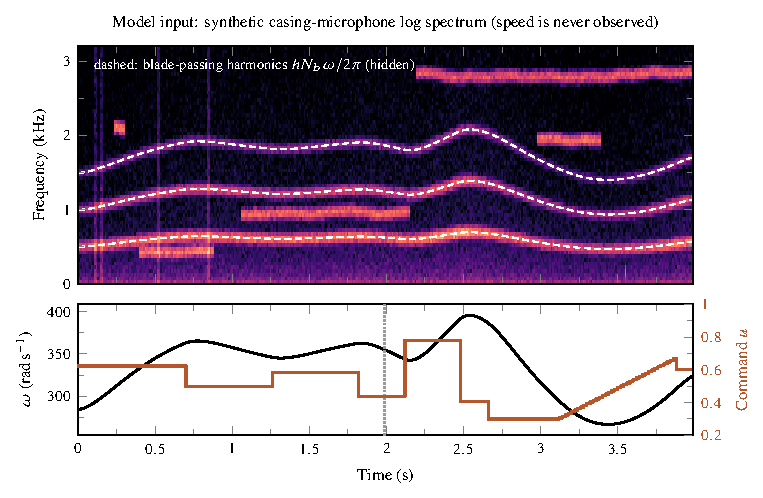
\includegraphics[width=0.72\textwidth]{fig_problem.pdf}
\caption{One test episode. Top: the model input, with the hidden blade-passing harmonics overlaid for illustration. Bottom: the hidden rotor speed and the known command. Forecasts start at $t=\SI{2}{\second}$.}
\label{fig:problem}
\end{figure*}

\subsection{Splits and protocol}
There are 3000 training and 300 validation episodes, and 300-episode test sets for the training distribution, the held-out regime and $\lambda\in\{0,0.5,1,2,3\}$. Each episode lasts \SI{4}{\second}. Models see the first \SI{2}{\second} of spectra and commands, then forecast the next \SI{2}{\second} open loop under the known future commands. Test sets are used only for reported numbers. Checkpoint selection, probe regularisation and controller tuning use validation data.

\section{Methods}\label{sec:method}
\subsection{Two-stage action-conditioned JEPA}
\emph{Stage 1} pre-trains a causal time--frequency CNN trunk $T_\theta$ (three $3\times5$ convolutions, causal in time) by masked latent prediction on 32-frame crops. Two or three time--frequency blocks and the final 3--8 frames are masked. A convolutional predictor maps the context features to the EMA trunk's per-position, layer-normalised features at the masked cells:
\begin{equation}
\mathcal L_1=\frac{1}{|M|}\sum_{(t,f)\in M}\big\lVert g_\psi(T_\theta(x\odot\bar M))_{tf}-\mathrm{LN}(T_{\bar\theta}(x))_{tf}\big\rVert_1,
\end{equation}
with $\bar\theta\leftarrow m\bar\theta+(1-m)\theta$ and $m$ following a cosine schedule from 0.996 to 1. This stage uses no actions and no labels.

\emph{Stage 2} freezes the trunk. A trainable spatial-soft-argmax readout~\cite{finn2016spatial} and a GRU turn the trunk features and past commands into a layer-normalised belief $z_t\in\mathbb R^{48}$. A residual predictor $z_{t+1}=\mathrm{LN}(z_t+f_\phi(z_t,u_t))$ is rolled out for $K$ steps, and a head $q$ must match the frozen, frequency-pooled trunk maps $y_{t+k}$ of the future frames:
\begin{equation}
\begin{aligned}
\mathcal L_2={}&\sum_{k=0}^{K}\big\lVert q(P^k_\phi(z_t,u_{t:t+k}))-y_{t+k}\big\rVert_1\\
&+\beta\sum_{k=1}^{K}\big\lVert P^k_\phi(z_t,\cdot)-\mathrm{sg}(z_{t+k})\big\rVert_2^2,
\end{aligned}
\end{equation}
plus one-step teacher forcing. The second term is TD-MPC2's latent consistency~\cite{hansen2024tdmpc2}, with $\beta=1$, applied identically to every learned method. The main configuration uses $K=128$ (\SI{1.28}{\second}) on \SI{3.2}{\second} training crops. Because the targets come from a frozen trunk that sees only observations, the latent cannot collapse onto the command history (Sec.~\ref{sec:failures}).

\emph{Read-out and use.} Speed is decoded by a frozen ridge probe, or by an MLP probe where stated, fitted on $N$ labelled training episodes. Forecasts decode open-loop latent rollouts through the same probe. Control authority $\partial\hat\omega/\partial u$ is a central finite difference through the rollout. Planning uses cross-entropy-method model predictive control (CEM-MPC) in latent space with a \SI{0.5}{\second} horizon. \emph{JEPA + fine-tune} trains the whole JEPA world model on the supervised loss below.

\begin{figure*}[!t]\centering
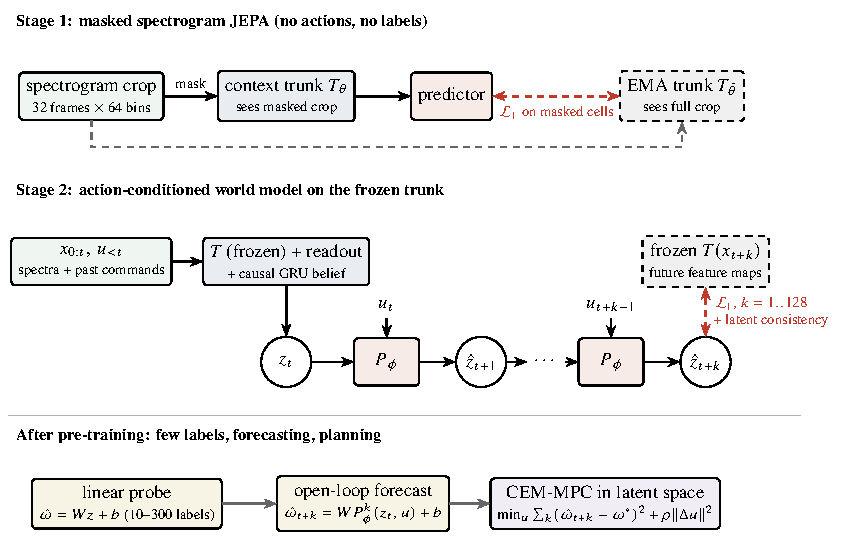
\includegraphics[width=0.84\textwidth]{fig_architecture.pdf}
\caption{Two-stage action-conditioned JEPA. Stage 1 learns spectrogram features by masked latent prediction. Stage 2 freezes them and learns action-conditioned latent dynamics by predicting future frozen feature maps. A few labels then suffice for a probe that supports forecasting and latent-space MPC.}
\label{fig:arch}
\end{figure*}

\subsection{Controls}
All learned controls share the trunk architecture, readout, belief encoder, predictor, optimiser (AdamW with a cosine schedule), batch, crops, rollout length, consistency term and step budget. They differ only in the training signal:
\begin{itemize}
\item \emph{Reconstruction world model}: every encoded and predicted latent is decoded back to the 64-bin spectrum (MSE), as in observation-prediction world models~\cite{hafner2019planet}.
\item \emph{Supervised}: the true speed is regressed from every encoded and predicted latent, with 10--3000 labelled episodes and early stopping on labelled validation error. This is the only method given label-based checkpoint selection.
\item \emph{Classical pipeline}: a three-harmonic comb tracker with Viterbi smoothing under a slew limit, tuned on validation, is followed by batched output-error identification of the \emph{true} form of~\eqref{eq:truth} with a delay search, and then by simulation. This pipeline is given knowledge the learned models do not have.
\end{itemize}
We also report nominal physics with catalogue parameters, persistence, an oracle with the true parameters and state, a PI controller on the tracked speed with gains tuned on validation, and a random-encoder probe.

\section{Results}\label{sec:results}
Unless stated otherwise, errors are rotor-speed RMSE in \si{\radian\per\second} over 300 test episodes. The JEPA, reconstruction and fully supervised world models in the main configuration report the mean $\pm$ s.d.\ over \nSeeds{} seeds. The supervised label sweep, JEPA + fine-tune, the closed-loop study, the hybrid and all ablations use seed 0, and the text compares seed-0 numbers with seed-0 numbers.

\subsection{Forecasting and state estimation}
Table~\ref{tab:main} and Fig.~\ref{fig:horizon} summarise accuracy. The oracle reproduces the stored trajectories exactly, which verifies the protocol. Nominal physics (\nNominalH{} at \SI{2}{\second}) shows how much the hidden parameters matter. With a 300-label linear probe, the JEPA world model forecasts \SI{2}{\second} ahead with \nJepaH{}, against \nReconH{} for the reconstruction world model trained identically. With MLP probes the figures are \nJepaMlpH{} and \nReconMlpH{}. JEPA + fine-tune reaches \nFtThreeH{} with 300 labels, against \nSupThreeH{} for supervised training from scratch on the same labels. Full supervision with 3000 labels reaches \nSupAllH{}. The classical pipeline, given the exact equation, remains the most accurate in distribution at \nGreyH{}. For state estimation, the MLP-probed JEPA belief (\nJepaMlpFilt{}) is on par with the hand-built tracker (\nTrackerFilt{}).

\begin{table*}[!t]\centering\scriptsize
\caption{Main results. Rotor-speed RMSE in \si{\radian\per\second} (mean $\pm$ s.d.\ over seeds), RMS torque residual of the forecast under the true parameters in \si{\newton\metre}, and median relative error of the \SI{2}{\second} control gain.}
\label{tab:main}
\tablefile{main}
\end{table*}

\begin{figure*}[!t]\centering
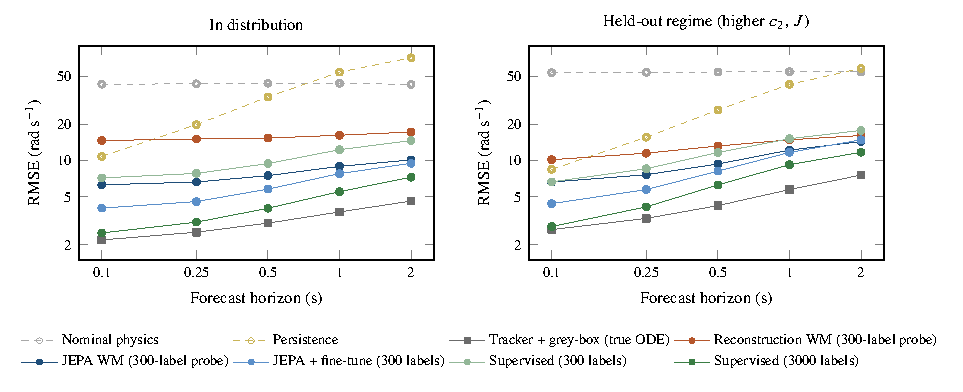
\includegraphics[width=0.92\textwidth]{fig_horizon.pdf}
\caption{Forecast error against horizon, in distribution (left) and in the held-out regime (right). Bands span seeds.}
\label{fig:horizon}
\end{figure*}

\subsection{Label efficiency}
Fig.~\ref{fig:labels} shows the result that matters most when labels are expensive. With ten labelled episodes, a linear probe on the frozen JEPA latent forecasts with \nJepaProbeTen{} (mean over three pre-training seeds), against \nSupTen{} for the same network trained from scratch on those ten episodes (seed 0; a factor of \nLabelRatioTen). JEPA pre-training followed by fine-tuning beats supervised training at every budget up to 300 episodes. Supervision overtakes the frozen probe only when labels are plentiful.

\begin{figure*}[!t]\centering
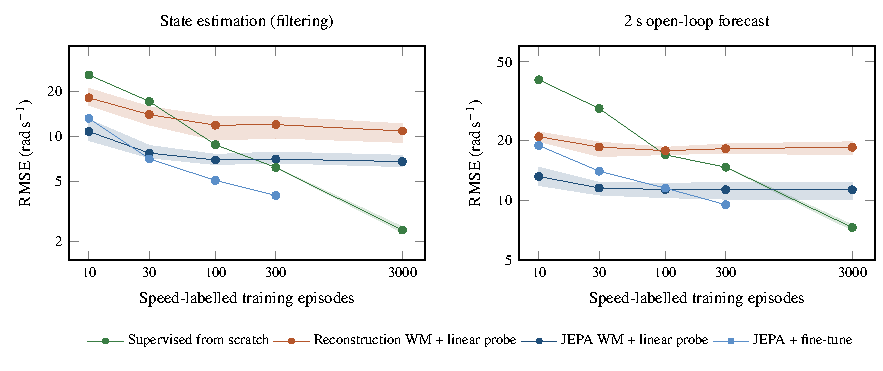
\includegraphics[width=0.92\textwidth]{fig_labels.pdf}
\caption{Filtering and \SI{2}{\second} forecast error against the number of speed-labelled training episodes. The self-supervised models also see all 3000 unlabelled episodes.}
\label{fig:labels}
\end{figure*}

\subsection{Robustness to nuisance and regime shift}
The comb tracker locks onto distractor tones once they are frequent (Fig.~\ref{fig:nuisance}, $\lambda\geq2$). As a result, the classical forecast degrades from \nGreyLamZero{} at $\lambda=0$ to \nGreyLamThree{} at $\lambda=3$. The JEPA world model, trained only at $\lambda=1$, degrades from \nJepaLamZero{} to \nJepaLamThree{}, and the reconstruction world model reaches \nReconLamThree{}. With 300 labels, JEPA + fine-tune holds \nFtThreeLamThree{} at $\lambda=3$, while supervised training from scratch reaches \nSupThreeLamThree{}. In the held-out dynamical regime the JEPA forecast rises to \nJepaOOD{} and the grey-box forecast to \nGreyOOD{}.

\begin{figure*}[!t]\centering
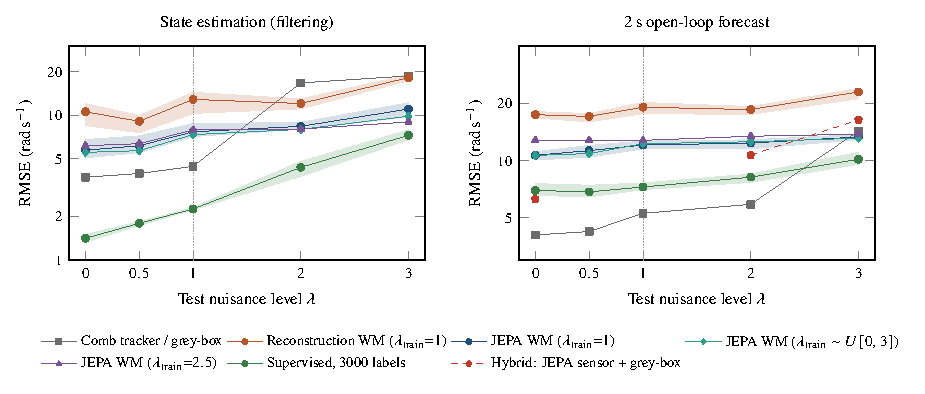
\includegraphics[width=0.92\textwidth]{fig_nuisance.pdf}
\caption{Filtering and forecast error against test nuisance $\lambda$ (dotted line: training level), with 300-label linear probes for the self-supervised models. Learned models are trained at $\lambda=1$ unless marked. The hybrid is seed 0.}
\label{fig:nuisance}
\end{figure*}

\subsection{Control authority and hidden parameters}
Every learned model now reproduces the plant's step response to a command change (Fig.~\ref{fig:step}), the property whose absence was the main v1 failure. The median relative error of the \SI{2}{\second} gain is \nGainJepa{} for JEPA, \nGainRecon{} for reconstruction, \nGainSup{} for full supervision and \nGainGrey{} for the grey-box. This follows from training on time-varying commands, not from an architectural trick. Linear probes on $z_{t=\SI{2}{\second}}$ (Fig.~\ref{fig:probes}) recover the steady-state gain well ($R^2$ of \nRtwoKwJepa{} for $k_\omega$) and the actuator lag partly (\nRtwoTauJepa{}, and \nRtwoTauSup{} for supervision). They recover almost nothing of the inertia ($R^2$ of \nRtwoJJepa{}), the mass flow or the delay. The latent captures \emph{state} better than it \emph{identifies the machine}, and this is the main reason the true-structure grey-box still wins on long in-distribution forecasts.

\begin{figure*}[!t]\centering
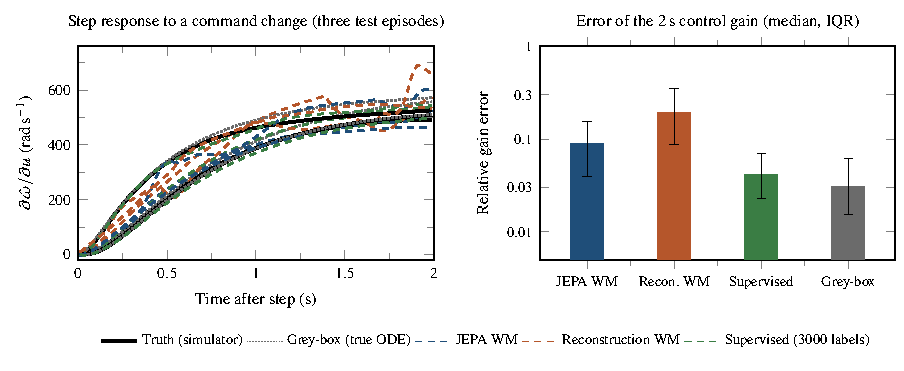
\includegraphics[width=0.92\textwidth]{fig_step.pdf}
\caption{Left: model step responses $\partial\hat\omega/\partial u$ (dashed) against simulator finite differences (black) for three test episodes. Right: median and interquartile range of the relative error of the \SI{2}{\second} gain over the test set.}
\label{fig:step}
\end{figure*}

\begin{figure}[!t]\centering
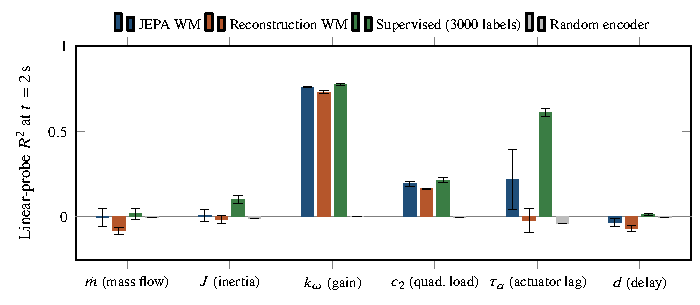
\includegraphics[width=\columnwidth]{fig_probes.pdf}
\caption{Linear-probe $R^2$ for the six hidden parameters (mass flow, inertia, gain, quadratic load, actuator lag and delay) from the belief at $t=\SI{2}{\second}$, with 300 labelled episodes.}
\label{fig:probes}
\end{figure}

\subsection{Closed-loop control by planning in latent space}
CEM-MPC controllers that differ only in their model track moderate set-point steps from the spectrogram alone (Fig.~\ref{fig:mpc}). We report the excess tracking MSE over an oracle controller, with paired bootstrap intervals over 40 episodes. Planning through the JEPA latent with a 300-label probe gives an excess of \nMpcJepaId{}\,\si{\radian\squared\per\second\squared}, close to the true-structure grey-box (\nMpcGreyId{}). With 300 labels, JEPA pre-training gives \nMpcFtId{}, against \nMpcSupThreeId{} for supervised training from scratch (a factor of \nMpcRatioId). At $\lambda=3$ the gap widens to \nMpcFtLamThree{} against \nMpcSupThreeLamThree{} (a factor of \nMpcRatioLamThree). A PI controller on the tracked speed is far worse (\nMpcPiId{}) and fails when the tracker fails (\nMpcPiLamThree{}, Fig.~\ref{fig:trace}).

\begin{figure*}[!t]\centering
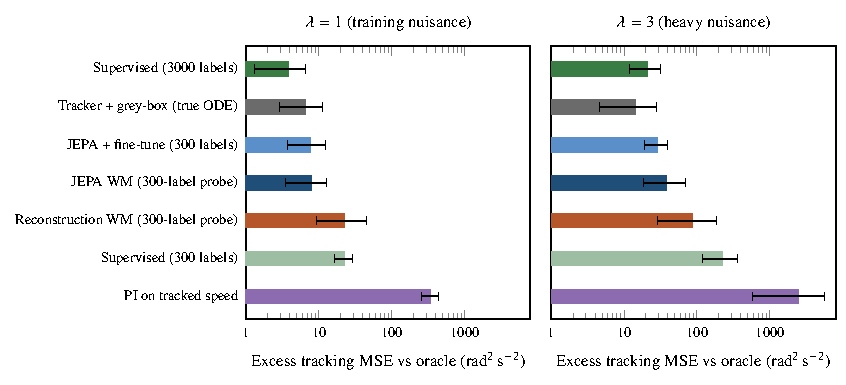
\includegraphics[width=0.74\textwidth]{fig_mpc.pdf}
\caption{Closed-loop excess tracking MSE over the oracle (40 test episodes, paired bootstrap 95\% CIs) at the training nuisance (left) and heavy nuisance (right).}
\label{fig:mpc}
\end{figure*}

\begin{figure}[!t]\centering
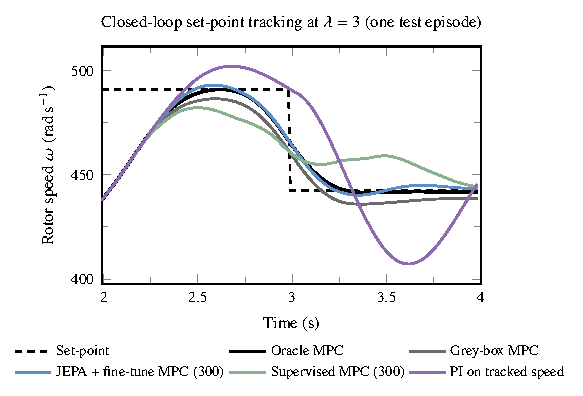
\includegraphics[width=\columnwidth]{fig_mpc_trace.pdf}
\caption{One closed-loop episode at $\lambda=3$. The PI controller acts on a tracker that has locked onto a distractor.}
\label{fig:trace}
\end{figure}

\section{Failure modes met during development}\label{sec:failures}
\emph{Action shortcut.} A single-stage action-conditioned JEPA whose EMA target encoder also received the commands collapsed to an effective latent rank of 2.6 of 48 within a few hundred steps (Fig.~\ref{fig:collapse}). Its speed probe stayed at the level of an untrained encoder. The latent encoded only the command history, which an action-conditioned predictor forecasts perfectly. VICReg-strength variance and covariance terms~\cite{bardes2022vicreg} did not prevent this, but targets that see only observations did. We expect the same shortcut in any self-predictive world model whose target encoder sees the actions~\cite{schwarzer2021spr}.

\emph{Read-out bottleneck.} An untrained soft-argmax read-out discarded the speed information. An MLP probe on the full trunk map reached \SI{5.1}{\radian\per\second}, against \SI{18.1}{\radian\per\second} on the read-out, so the read-out is trained in stage 2.

\emph{Rollout drift.} Without the consistency term, probe-decoded rollouts diverged beyond the training horizon.

\emph{Infeasible control task.} The first closed-loop task used set-point steps of up to 80\% of the reachable band. Every controller, the oracle included, was saturation-limited, so the task measured the actuator rather than the model. It was replaced by moderate steps, and the old results are archived.

\begin{figure*}[!t]\centering
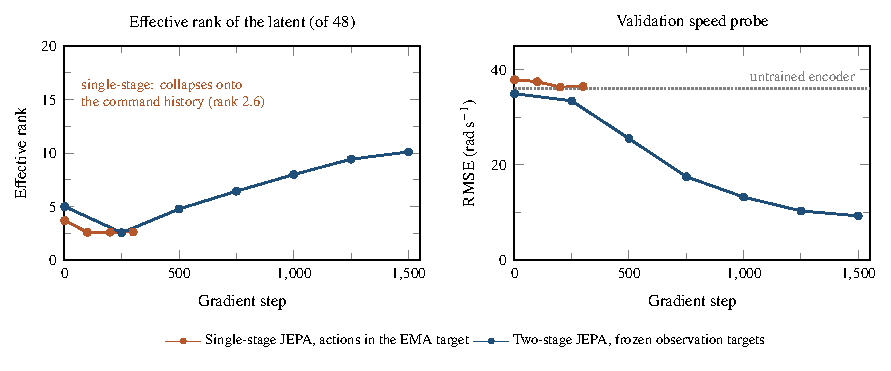
\includegraphics[width=0.92\textwidth]{fig_collapse.pdf}
\caption{Action-shortcut collapse. A single-stage JEPA whose EMA target sees the commands collapses (left) and never learns speed (right). The two-stage design with frozen observation targets does not.}
\label{fig:collapse}
\end{figure*}

\section{Second-round improvements}\label{sec:round2}
The first-round results suggested four targeted changes, each aimed at one finding. Fig.~\ref{fig:ablation} collects them with the original ablations. All numbers in this section are seed 0.

\emph{Training horizon.} Increasing the rollout length from 0.64 to \SI{1.28}{\second} reduced the \SI{2}{\second} error from \nAblShort{} to \nJepaSzH{}. This is the largest single gain in the study, and it helped every objective. Training on the full \SI{2}{\second} horizon (\SI{4}{\second} crops) did \emph{not} help further: \nAblXlong{} in distribution, \nXlongOOD{} in the held-out regime and \nXlongLamThree{} at $\lambda=3$. The benefit of longer rollouts saturates, and fewer anchors per crop at that length is a plausible cost.

\emph{Nuisance-randomised pre-training.} Drawing $\lambda\sim U[0,3]$ per training episode, a form of domain randomisation~\cite{tobin2017domain}, splits cleanly by task. Perception became much more robust: with the MLP probe, filtering error at $\lambda=3$ fell from \nJepaSzMlpFiltLamThree{} to \nMixMlpFiltLamThree{}, and to \nHiMlpFiltLamThree{} when trained at a fixed $\lambda=2.5$. Forecasts barely moved (\nJepaSzMlpLamThree{} against \nMixMlpLamThree{} at $\lambda=3$, and \nAblMix{} in distribution with the linear probe). Seeing the speed better does not fix the long-horizon error, which again points at dynamics and identification rather than perception. In closed loop at $\lambda=3$, planning with the $\lambda=2.5$-trained JEPA reduced the excess error from \nMpcJepaLamThree{} to \nMpcJepaHiLamThree{}.

\emph{JEPA perception with physics dynamics.} The causal JEPA belief, read by the MLP probe, replaced the comb tracker as the input to grey-box identification of the true equation, fitted from $t=\SI{0.3}{\second}$ (Fig.~\ref{fig:hybrid}). In distribution the hybrid forecasts with \nHybJepaId{}, against \nJepaSzH{} for the JEPA world model alone, a 30\% reduction. A tracker fitted over the same window does better (\nHybTrackerId{}), because its Viterbi track is smoothed offline while the JEPA belief is causal. At $\lambda=3$ the ordering reverses: the hybrid (\nHybJepaLamThree{}) beats the tracker over the same window (\nHybTrackerLamThree{}) but loses to the pure JEPA world model (\nAblJepaSzLamThree{}). Output-error identification amplifies sensor error, so physics dynamics pay off only when perception is good.

\emph{Seed ensembles.} A three-member ensemble of JEPA world models forecasts with \nEnsJepaId{}, against \nEnsSingleJepaId{} for a single member on average, and with \nEnsJepaLamThree{} against \nEnsSingleJepaLamThree{} at $\lambda=3$~\cite{lakshminarayanan2017ensembles}. The ensemble is over-confident, however. Only \nEnsCovJepaId\% of errors fall within $\pm2\sigma$ of the ensemble mean (\nEnsCovJepaOOD\% in the held-out regime), and spread and error correlate at only \nEnsCorrJepaId{} (Fig.~\ref{fig:spread}). The spread ranks difficulty weakly, but it is not a calibrated uncertainty.

\emph{Adaptive context and pre-training.} An explicit context embedding of recent transitions~\cite{lee2020cadm} made forecasts worse (\nAblCtx{}). Removing stage-1 pre-training cost \nAblRand{} against \nAblShort{} (both at the short horizon).

\begin{figure*}[!t]\centering
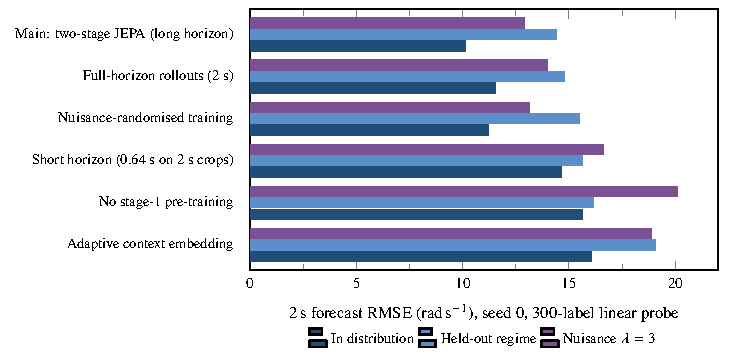
\includegraphics[width=0.70\textwidth]{fig_ablation.pdf}
\caption{Seed-0 ablations and second-round variants: \SI{2}{\second} forecast RMSE in distribution, in the held-out regime and at $\lambda=3$.}
\label{fig:ablation}
\end{figure*}

\begin{figure*}[!t]\centering
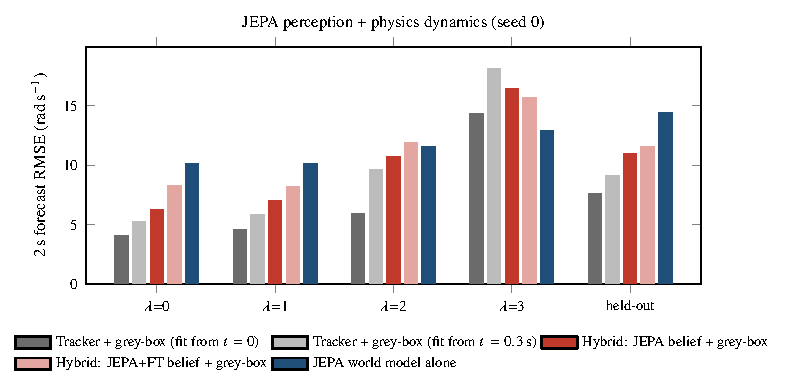
\includegraphics[width=0.78\textwidth]{fig_hybrid.pdf}
\caption{JEPA perception with physics dynamics (seed 0). Grey-box identification of the true equation driven by the comb tracker or by the causal JEPA belief, against the JEPA world model alone.}
\label{fig:hybrid}
\end{figure*}

\begin{figure*}[!t]\centering
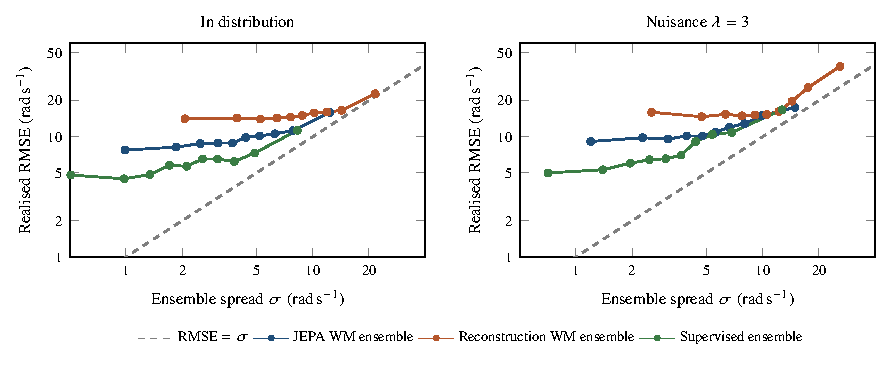
\includegraphics[width=0.92\textwidth]{fig_spread_skill.pdf}
\caption{Spread and skill of three-seed ensembles. Points below the dashed line would mean the spread over-states the error. All ensembles lie above it, so they are over-confident.}
\label{fig:spread}
\end{figure*}

\section{Discussion}
\emph{What JEPA buys here is labels and robustness, not peak accuracy.} When the equation of motion is known and the sensor is clean, a hand-built tracker plus grey-box identification is still the best forecaster in this study. The JEPA world model wins where that pipeline is brittle or expensive. It needs only a handful of labelled runs, it degrades gracefully as acoustic nuisance grows, and it supports planning directly in latent space. With 300 labels, JEPA pre-training reduced the excess closed-loop error by a factor of \nMpcRatioId{} at the training nuisance and \nMpcRatioLamThree{} under heavy nuisance.

\emph{Predicting representations beats predicting observations here.} With identical architecture, data and budget, the JEPA objective gave a far more linearly accessible speed estimate than reconstruction (\nJepaH{} against \nReconH{} at \SI{2}{\second} with linear probes), better control authority and better robustness. Under MLP probes the gap shrinks to \nJepaMlpH{} against \nReconMlpH{}. Much of the advantage is therefore in \emph{how} the information is organised, as well as \emph{whether} it is present.

\emph{The bottleneck is identifying the system, not perceiving it.} The belief recovers state about as well as a specialised tracker, and nuisance randomisation made perception markedly more robust. Yet long-horizon forecasts barely moved, and the latent recovers almost nothing of the inertia, mass flow or delay. Self-supervised world models need a stronger incentive for in-context system identification before they can rival structure-aware physics on extrapolation.

\section{Implications for learned turbulence closures and physics-informed models}\label{sec:implications}
The rotor is a toy, but each finding maps onto a concrete question for turbulence modelling. Table~\ref{tab:mapping} summarises the correspondence, and the paragraphs below explain it.

\begin{table}[!t]\centering\footnotesize
\caption{From the toy model to the closure problem.}
\label{tab:mapping}
\begin{tabular}{@{}p{0.43\columnwidth}p{0.49\columnwidth}@{}}
\toprule
Rotor toy model & Turbulence closure analogue\\
\midrule
Spectrogram (speed never observed) & Resolved, filtered field (subgrid state never observed)\\
Hidden per-episode parameters & Flow regime and local subgrid statistics\\
Speed labels from a tachometer & Filtered direct-simulation data\\
Known commands & Forcing, boundary and inflow conditions\\
Open-loop latent rollout & \emph{A posteriori} use inside a solver\\
Distractor tones & Measurement and discretisation noise\\
\bottomrule
\end{tabular}
\end{table}

\emph{Labels are the expensive part.} A closure label usually means a filtered direct simulation, whose cost grows steeply with Reynolds number~\cite{pope2000turbulent}. Learned large-eddy closures~\cite{beck2019les,maulik2019subgrid} and data-augmented Reynolds-averaged models~\cite{duraisamy2019turbulence,duraisamy2021perspectives} are therefore label-limited. The largest effect in this study is label efficiency: a probe on a self-supervised latent matched what supervision needed far more labels to reach. The analogous experiment is to pre-train a JEPA on plentiful coarse or large-eddy data, which costs no direct simulation, and then fit a closure head on a few filtered direct-simulation snapshots.

\emph{Predict representations of what is resolvable.} Reconstruction-based training must reproduce every unpredictable detail of the target, which for turbulence includes the chaotic small scales. JEPA's advantage over reconstruction here came from organising the predictable structure, not from storing more information. For closures, this suggests predicting representations of the future resolved field rather than reconstructing it. Whether those representations then carry the subgrid information a closure needs is the central open question.

\emph{Train the way the model will be used.} Long-rollout training gave the largest single gain, then saturated. This echoes the closure literature's gap between \emph{a priori} accuracy and \emph{a posteriori} behaviour inside a solver~\cite{duraisamy2021perspectives,beck2019les}. Kochkov \emph{et al.}~\cite{kochkov2021mlcfd} closed that gap by training through the unrolled solver. A JEPA closure should be trained on rollouts of the coupled model, not on single-step targets.

\emph{Never let the target see the forcing.} The action-shortcut collapse is a warning for any self-predictive closure. If the target encoder sees the forcing, boundary or inflow conditions, a predictor that is also given them can satisfy the loss without learning the flow. Targets built only from the flow field avoid this.

\emph{Physics constraints help only when perception is good.} The hybrid cut the in-distribution error by 30\% but amplified sensor error under heavy nuisance. PINNs face a related problem: equation residuals are a strong prior, but their optimisation is fragile and can fail on harder regimes~\cite{krishnapriyan2021failure,wang2021gradient}. The lesson is to place physics where the inputs are reliable, for example as structure in the predictor, rather than as a fit to noisy estimates.

\emph{State is not identification.} The latent recovered the rotor's state but only part of its parameters. For turbulence, recovering the resolved state is not enough: a closure must also infer regime-dependent statistics from the flow's history. This is exactly the question the ``What the Grid Can't See'' study asks.

\emph{Uncertainty must be calibrated.} The ensembles were over-confident. A closure that reports its own uncertainty is only useful in a solver if that uncertainty is calibrated~\cite{lakshminarayanan2017ensembles}.

\emph{Roadmap.} These points suggest a staged test of JEPA for turbulence:
\begin{enumerate}
\item pre-train a masked space--time JEPA on coarse fields of a canonical flow, such as decaying isotropic turbulence or channel flow, with no subgrid labels;
\item probe the frozen latent for filtered subgrid stresses with a few filtered direct-simulation snapshots, and compare against supervised closures~\cite{beck2019les,maulik2019subgrid};
\item train the predictor through rollouts of the coupled coarse solver and evaluate \emph{a posteriori}~\cite{kochkov2021mlcfd};
\item compare JEPA encoders with neural-operator backbones~\cite{li2021fno,lu2021deeponet}, and with PINN-style residual terms~\cite{raissi2017pinn} added only to the predictor;
\item calibrate ensemble uncertainty before any closure is coupled to a solver.
\end{enumerate}
If the toy-model pattern holds, the expected payoff is a closure that needs far fewer high-fidelity labels and tolerates noisy inputs. Its accuracy may still trail a closure with the right physical structure in regimes where that structure is known.

\section{Limitations and claim boundary}
Everything here is synthetic. The truth model is a scalar rotor with a first-order actuator, the sensor is a declared spectral model rather than a measured microphone, and the distractors are stylised. The classical pipeline is given the exact model structure, which a real engine does not offer. The learned models are given 3000 unlabelled episodes of system-identification excitation, which a test cell might or might not provide. The closed-loop study, the hybrid, the supervised label sweep and all second-round variants rest on a single seed, and the supervised and fine-tuned label-sweep runs for seeds 1 and 2 were dropped for compute reasons. A scalar rotor is far simpler than a turbulent flow, so the mapping in Sec.~\ref{sec:implications} motivates experiments rather than predicting their outcome. The results establish what this JEPA formulation can and cannot recover under controlled, fully known conditions. They validate no engine, sensor, controller or turbulence closure.

\section{Conclusion}
Rebuilt around a partially observed, action-driven rotor, a two-stage action-conditioned JEPA learns a useful world model from unlabelled sound. With ten labelled episodes it forecasts \nLabelRatioTen{} times better than supervised training from scratch. It tolerates acoustic nuisance that breaks a hand-built tracker, recovers control authority, and plans close to an oracle. It does not match a classical pipeline that is given the true equation in distribution, and its latent identifies the system only partly. As a toy test of JEPA for physics, the result is encouraging on labels and robustness and sobering on identification. Both findings point to the experiments needed before JEPA is applied to recovering unresolved turbulence.

\bibliographystyle{IEEEtran}
\bibliography{references}
\end{document}
